\subsection{Estágio no Exterior}

O estágio contou com o apoio financeiro da CNPQ (Processo: 241028/2012-4) e foi realizado no \textit{Institut national de recherche en informatique et en automatique} (INRIA), França. O aluno ficou na França por um ano (Abril de 2013 - Abril de 2014) sob a supervisão do professor Doutor Nicolas Anquetil. O grupo de pesquisa é especializado em remodularização e modernização de sistemas orientados a objetos com enfoque em \textit{Model-Driven Development}. 

Dois projetos foram conduzidos durante a estadia na França, descritos nas Seções X e Y. É importante enfatizar que ambos os projetos são diretamente relacionados à realização deste projeto de doutorado.

O vínculo com o CNPQ foi encerrado no mês de Abril e a bolsa da FAPESP foi reatividade. Uma cópia do parecer emitido pelo orientador no exterior pode ser encontrado no Apêndice A.

\subsection{Mapeamento Sistemático}

Quando se conduz uma revisão de literatura sem o pré-estabelecimento de um protocolo de revisão há um direcionamento por interesses pessoais, o que leva a resultados pouco confiáveis. Neste contexto, pesquisadores vem utilizando uma técnica denominada de Mapeamento Sistemático (MS) para auxiliar o pesquisador a conduzir um revisão bibliográfica de forma totalmente sistemática com o intuito de evitar que trabalhos importantes fiquem fora de suas pesquisas. Um MS é caracterizada por ser um meio de avaliar e interpretar todas as pesquisas disponíveis, referentes a um questão de pesquisa, tema, área ou fenômeno de interesse. O MS tem como objetivo apresentar uma avaliação justa de um tema de pesquisa, utilizando uma metodologia confiável, rigorosa e auditável~\cite{kit04}.

De acordo com~\citet{kit04} o MS implica na forma mais adequada para se identificar, avaliar e interpretar toda pesquisa importante para um tema em particular. Resume-se que um MS configura um alicerce para novas atividades de pesquisa acerca de determinado tema. Dessa forma, foi realizado um MS sobre \textit{Architecture-Driven Modernization} (ADM) e \textit{Knowledge-Discovery Metamodel} (KDM). A nossa motivação para realizar esse MS é identificar os temas que têm sido mais investigados, bem como os temas que ainda não foram investigados. Embora, a ADM é uma abordagem relativamente nova, OMG afirma que ela é uma importante abordagem pois combina dois dos principais campos da Engenharia de Software, ou seja, \textit{Model-Driven Development} e Engenharia Reversa. Desde a definição da ADM muitos esforços têm enfatizado a modernização de sistemas legados por meio desta abordagem. Neste contexto, é importante realizar uma investigação mais sistemática dos temas englobados por esta área de pesquisa. 

Para atingir este objetivo, foi realizado um MS. Os resultados, bem como o protocolo de pesquisa elaborado, foram publicados no \textit{IEEE Information Reuse and Integration} (IRI 2014) , o qual tem qualis B2. O artigo foi apresentado pelo bolsista em Agosto de 2014 em São Francisco, California. Maiores detalhes sobre esse artigo pode ser obtido no Apêndice A deste relatório. O mesmo anexo contem uma cópia da obra submetida.


\subsection{Estabelecimento do Catalogo de Refatoração para o metamodelo KDM} % (fold)
	 \label{sub:catalogo_kdm}

Foi elaborado um catalogo dedicado para ser aplicado no metamodelo do KDM. Mais especificamente esse catalogo foi adaptado com base em catálogos já disponíveis na literatura. Para a definição desse catalogo de refatoração, foi utilizado um formato inspirado pelo~\cite{refactImpro}. Em outras palavras, o catalogo foi descrito da seguinte forma: (\textit{i}) o nome do refatoração, (\textit{ii}) descrição da típica situação onde a refatoração deve ser aplicada, (\textit{iii}) descrição da solução para solucionar uma determinada situação problemática, (\textit{iv}) pre-condições que devem ser satisfeitas para aplicar a refatoração, (\textit{v}) os parâmetros necessários para executar a refatoração e (\textit{vi}) descrição dos passos para realizar a refatoração.

O catalogo de refatoração é estruturado em quatro grupos como pode ser observado na Tabela~\ref{tab:catalogue}, a qual contêm 17 refatorações. O primeiro grupo chamada \textit{Rename Feature} consiste de refatorações para renomear \textit{ClassUnit}, \textit{StorableUnits} e \textit{MethodUnits}. O segundo grupo, \textit{Moving Features Between Objects} consiste de refatorações simples, tais como mover ou criar características, ou seja, criar ou mover atributos, métodos ou classes. O terceiro grupo,  \textit{Organizing Data}, é responsável por definir um conjunto de refatorações para ser organizar a estrutura do código-fonte. Por fim, o quatro grupo, \textit{Dealing With Generalization}, representa refatorações para mover métodos e/ou atributos sobre uma especifica hierarquia de classes. 

\begin{table}[!h]
\caption{Refactorings Adapted to KDM}
\label{tab:adaptedRefactoring}
\centering
  % Requires \usepackage{graphicx}
  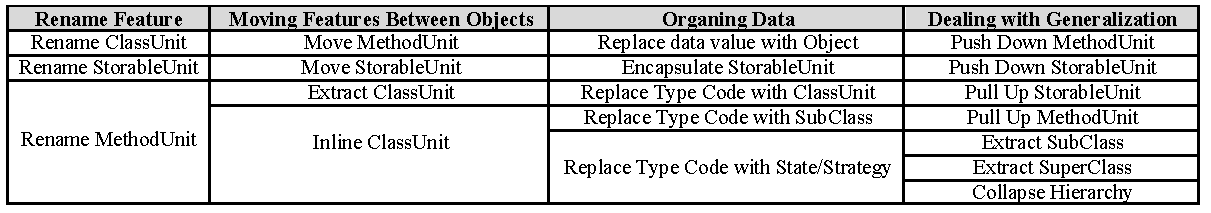
\includegraphics[scale=0.67]{figuras/NovoCatalogue}
\end{table}

Vale ressaltar que um artigo descrevendo o catalogo de refatoração adaptado para o KDM também foi no \textit{IEEE Information Reuse and Integration} (IRI 2014) , o qual tem qualis B2. O artigo foi apresentado pelo bolsista em Agosto de 2014 em São Francisco, California. Além disso, o bolsista participou das sessões técnicas e palestras. Maiores detalhes sobre esse artigo pode ser obtido no Apêndice B deste relatório. O mesmo contem uma cópia da obra submetida.

\subsection{Um ambiente integrado para desenvolvimento e apoio para o catalogo de refatorações do metamodelo KDM}

Durante a revisão sistemática pode-se averiguar que tanto o processo ADM e o seu metamodelo KDM têm sido vastamente utilizado na literatura para auxiliar a modernização de sistemas legados. No entanto, também pode-se verificar qua até o momento não existe nenhum ambiente integrado de desenvolvimento para guiar o engenheiro para automaticamente aplicar as refatorações e modernizações como existe em outros paradigmas, tais como o paradigma orientado a objetos. Para mitigar tal limitação, durante o período de vigência da bolsa foi desenvolvido um \textit{plug-in} utilizando a plataforma do Eclipse. 

Esse \textit{plug-in} fornece um ambiente para realizar as refatorações apresentadas na Seção~\ref{sub:catalogo_kdm} de forma totalmente automatizada. Na Figura~\ref{fig:ferramenta} é ilustrado todo o processo no qual o \textit{plug-in} é baseado. Como pode ser observado nessa figura a utilização do \textit{plug-in} pode ser ilustrada em três passos: (\textit{i}) engenharia reversa (\textit{reverse engineering}), (\textit{ii}) refatorações (\textit{refactorings}) e (\textit{iii}) engenharia avante (\textit{forward engineering}). Maiores detalhes sobre tais passos são descritos nas próximas seções.

\begin{figure}[!h]
 \centering
 \scalebox{0.6}{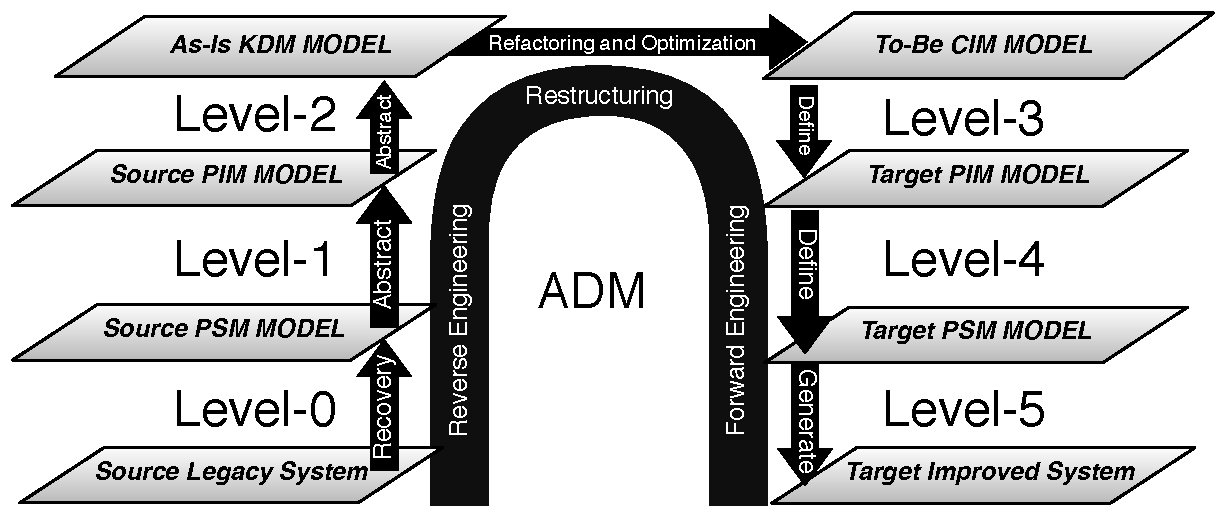
\includegraphics{figuras/processoDaFerramenta}}

\caption{Passos para utilização do \textit{plug-in}}
 \label{fig:ferramenta}
\end{figure}


 \subsubsection{Engenharia Reversa}

Para iniciar esse passo o engenheiro de software deve entrar com um arquivo que representa uma instância do metamodelo KDM ou um determinado código-fonte para realizar a refatoração. No caso do código-fonte ser a entrada escolhida, o engenheiro de software começa o processo no \textbf{Level-0} escolhendo um projeto no Eclipse\footnote{https://www.eclipse.org/} que contenha o código-fonte para realizar as refatorações. Posteriormente, no \textbf{Level-1} o código-fonte precisa ser transformado para um modelo especifico de plataforma (no inglês - Platform-Specific Model (PSM)). Esse PSM representa uma instância do código-fonte em um nível mais abstrato do código-fonte. Para realizar essa transformação (código-fonte para PSM) foi implementado um extrator de modelo em Java.

Após criar o PSM o próximo level (\textbf{Level-2}) consiste em transformar o PSM para um Modelo Independente de plataforma (no inglês - Platform-Indented Model (PIM)) o qual é baseado no metamodelo do KDM. Nesse level o \textit{plug-in} utiliza o \textit{framework} MoDisco\footnote{http://www.eclipse.org/MoDisco/} para realizar a transformação de PSM para PIM.

Na Figura~\ref{fig:plugin} é apresentado uma visão geral do \textit{plug-in} desenvolvido pelo bolsista durante a período de vigência da bolsa. Apenas para o propósito de explicação, foi identificado quatro principais regiões do \textit{plug-in}, veja Figura\ref{fig:plugin} \textcircled{a}, \textcircled{b}, \textcircled{c} and \textcircled{d}.

\begin{figure}[!h]
 \centering
 \scalebox{0.9}{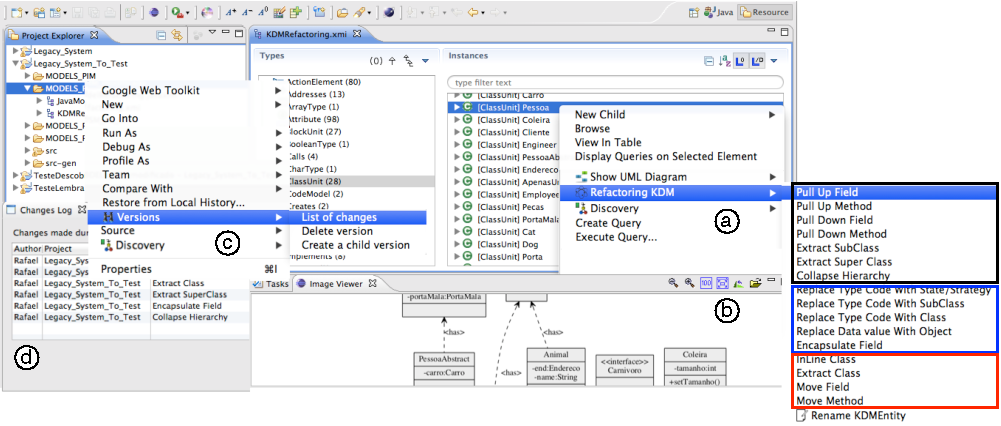
\includegraphics{figuras/ScreenShot_tool}}
\caption{Visão geral do \textit{plug-in} desenvolvido}
 \label{fig:plugin}
\end{figure}

Como já salientado anteriormente todas as refatorações fornecidas pelo \textit{plug-in} são feitas com base no metamodelo KDM. Dessa forma, para auxiliar o engenheiro de software a realizar as refatorações um menu chamado \textit{Refactoring KDM} foi adicionado, veja Figura~\ref{fig:plugin}\textcircled{a}. Utilizando esse menu o engenheiro de software pode interagir com o metamodelo do KDM e escolher qual refatoração deve ser executada. Note que na região \textcircled{a} da Figura~\ref{fig:plugin} é possível ver todas as 17 refatorações implementadas no \textit{plug-in}.

Na região \textcircled{b} da Figura~\ref{fig:plugin} é apresentado um diagrama de classe. Esse diagrama pode ser utilizado pelo engenheiro de software antes ou depois de aplicar as refatorações no modelo KDM. Usualmente o engenheiro pode utilizar esse diagrama antes de aplicar refatorações para decidir onde deve-se realmente aplicar as refatorações. Além disso, esse diagrama é útil por que geralmente sistemas legados não contêm nenhum tipo de documentação, sendo o código-fonte o único artefato disponível do mesmo. Portanto, criar um diagrama de classe durante a execução de refatorações no sistema legado pode ser uma boa alternativa para melhorar a documentação de um determinado sistema.

O \textit{plug-in} também fornece múltiplas versões de um sistema em nível de modelos, ou seja, em nível de modelos KDM. O objetivo é permitir que o engenheiro de software trabalhe interativamente em vários modelos, permitindo assim que o engenheiro de software escolha e explore diferentes caminhos de refatoração. Como pode ser observado na região  \textcircled{c} da Figura~\ref{fig:plugin}, o engenheiro deve selecionar o arquivo KDM e escolher a opção ``\textit{Versions}''. Três opções são disponíveis nesse menu (\textit{i}) \textit{List of Changes}, (\textit{ii}) \textit{Delete version} and (\textit{iii}) \textit{Create a child version}. A primeira opção mostra todas refatorações que já foram feitas pelo engenheiro (ver região \textcircled{d} ) - a segunda opção é responsável por deletar uma versão - e a ultima opção criar uma cópia do arquivo KDM, permitindo assim que o engenheiro aplique outras refatorações e explore diferentes caminhos de refatoração sem afetar o modelo KDM principal do projeto.


 \subsubsection{Executando Refatorações no \textit{Plug-in}}

Após o engenheiro clicar no menu da região \textcircled{a} (ver Figura~\ref{fig:plugin}) e escolher qual refatoração aplicar um \textit{Wizard} será mostrado. Para explicação, considere que o engenheiro de software escolheu aplicar a refatoração denominada \textit{Extract Class}. Então o engenheiro deve selecionar qual metaclass o mesmo deseja extrair, esse passo é ilustrado na Figura~\ref{fig:wizard} (a). Posteriormente o \textit{plug-in} executa o \textit{Wizard} como ilustrado na Figura~\ref{fig:wizard} (b). Como pode ser observado, aqui o engenheiro de software pode atribuir um nome para a nova metaclasse. Além disso, uma prévia de todos os detectados \textit{StorableUnits} e \textit{MethodUnis} que podem ser extraídos e adicionados na outra classe também são mostrados. O engenheiro pode também selecionar se a nova classe será uma classe interna ou uma classe normal. Também é possível especificar se métodos assessores (\textit{getters} e \textit{setters}) devem ser criados ou não. 

\begin{figure}[!h]
 \centering
 \scalebox{0.6}{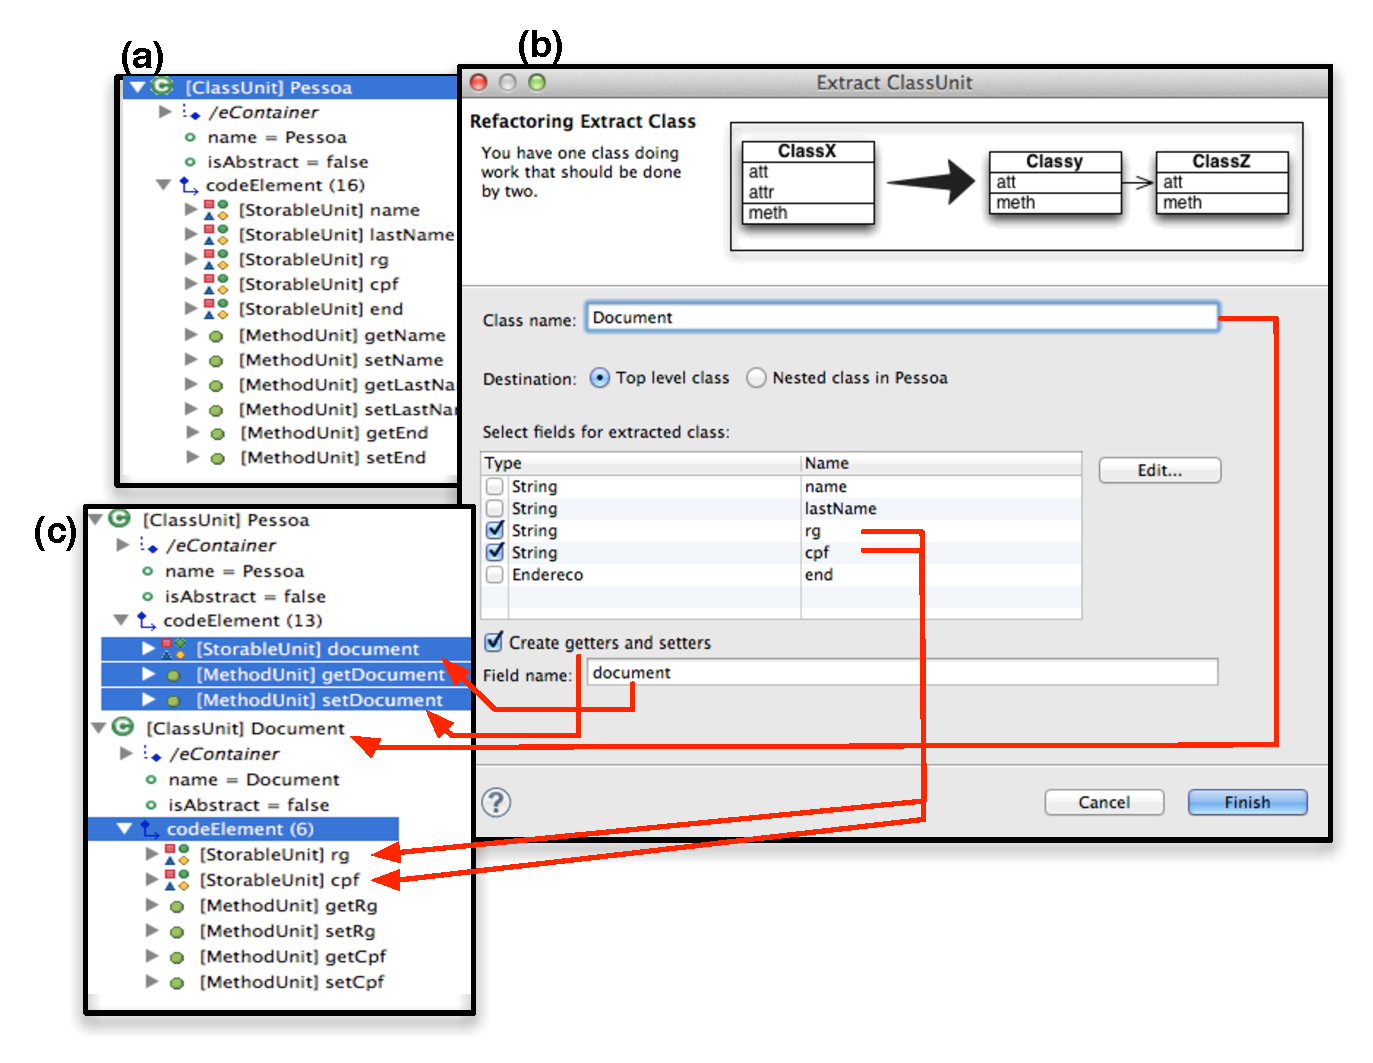
\includegraphics{figuras/Wizard2}}
\caption{Extract Class Wizard}
 \label{fig:wizard}
\end{figure}

Após o engenheiro preencher todos os campos necessários, ele pode clicar no botão \textit{Finish} e então a refatoração \textit{Extract Class} é executada. Como pode ser observado na Figura~\ref{fig:wizard} (c) uma nova instância de \textit{ClassUnit} denominada \textit{Document} foi criada - dois \textit{StorableUnits} da metaclasse \textit{Pessoa}, ``rg'' e ``CPF'' foram movidas para \textit{Document}.


 \subsubsection{Engenharia Avante}

Após o engenheiro realizar todas as refatorações no KDM os próximos passos são: (\textit{i}) transformar o KDM para um PSM e (\textit{ii}) transformar o PSM para artefatos físicos (código-fonte). O primeiro passo é executado baseado em um conjunto de transformações utilizando a linguagem ATL Transformation Languag (ATL)\footnote{https://www.eclipse.org/atl/}. O último passo consiste em utilizar \textit{templates} para gerar o código-fonte refatorado.  Na Figura~\ref{fig:forward} é apresentado como é feita a geração de código-fonte.

\begin{figure}[!h]
 \centering
 \scalebox{0.4}{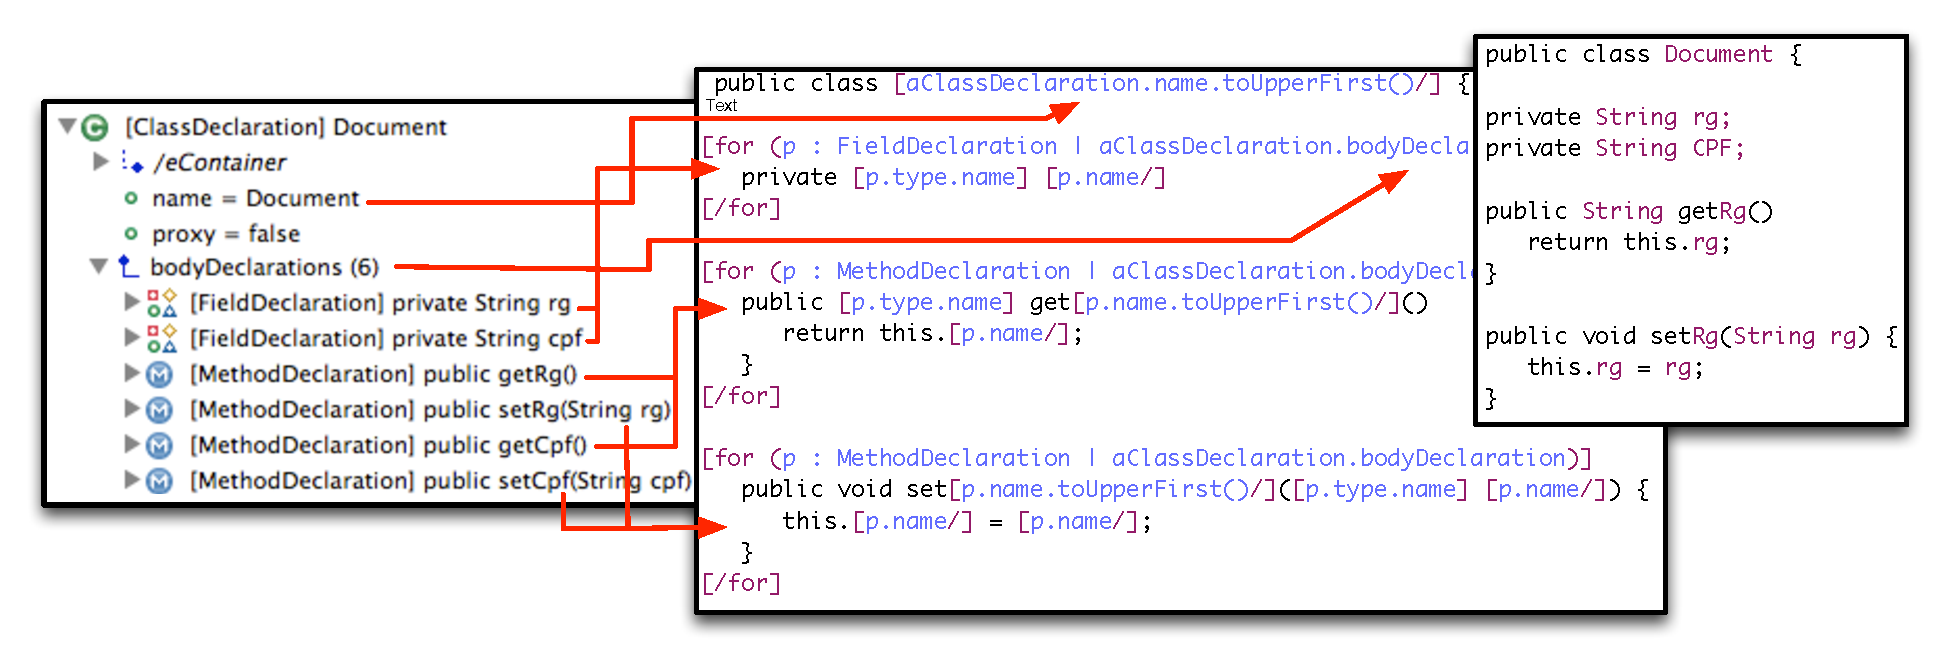
\includegraphics{figuras/ForwardEngineering}}
\caption{Passos da Engenharia Avante}
 \label{fig:forward}
\end{figure}

 \subsubsection{Arquitetura do \textit{plugin}}

Na Figura~\ref{fig:architecture} é ilustrado a arquitetura do \textit{plug-in} desenvolvido durante o período de vigência da bolsa. Como pode ser observado nessa figura, a primeira camada (\textit{layer}) é o \textit{Core Framework}. Essa camada representa que o \textit{plug-in} foi desenvolvida utilizando como base a plataforma de desenvolvimento Eclipse. Além disso, nessa camada pode-se observar que também foi utilizado Java e Groovy como linguagem de programação. Também é possível identificar que nessa camada alguns \textit{plug-ins} da plataforma de desenvolvimento Eclipse foram utilizados, tais como MoDisco\footnote{http://www.eclipse.org/MoDisco/} e EMF\footnote{https://www.eclipse.org/modeling/emf/}. Modisco e EMF ambos foram utilizados pois fornecem uma \textit{Application Programming Interface} (API) para facilitar o acesso ao metamodelo KDM.

\begin{figure}[!h]
 \centering
 \scalebox{0.8}{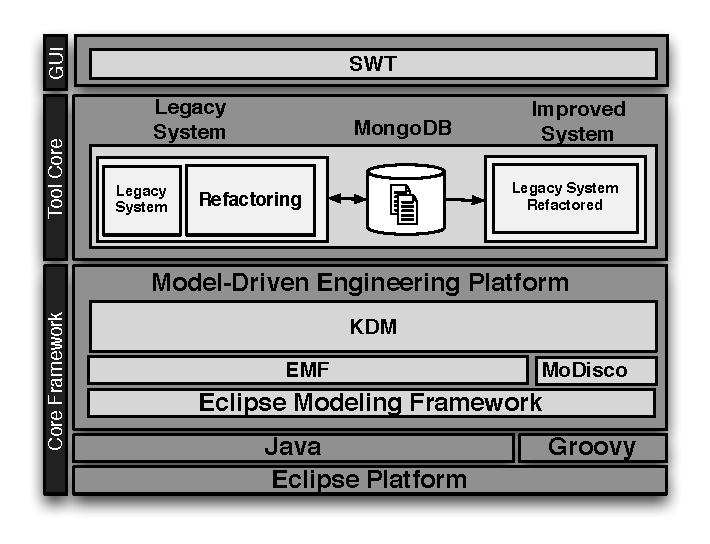
\includegraphics{figuras/Arquitetura}}
\caption{Arquitetura do \textit{plug-in}}
 \label{fig:architecture}
\end{figure}

A segunda camada, \textit{Tool Core}, é onde todas as refatorações fornecidas pelo \textit{plug-in} foram implementadas. A ultima camada é onde a interface gráfica do \textit{plug-in} foi desenvolvida. Vale ressaltar que um artigo sobre esse \textit{plugin} foi publicado no  2nd \textit{Workshop on Software Visualization, Evolution and Maintenance} (VEM). O bolsista esteve presente nesse evento, apresentado o artigo e participando das sessões técnicas e palestras. Mais detalhes sobre este \textit{plugin} podem ser encontrados na cópia desse artigo no Apêndice C.

\subsection{Um Metamodelo para Especificar Refatorações para o KDM - (\textit{Refac-KDM})}

Durante o desenvolvimento e evolução de software novas funcionalidades geralmente são adicionadas ou são ajustadas a novas exigências. Devido a tais alterações, a flexibilidade da arquitetura desse sistema pode ser um fator desafiador. Em outros casos, após aplicar um conjunto de alterações a arquitetura continua perfeitamente adequada. Porém, usualmente é necessário aplicar mudanças na arquitetura dessa sistema para confortar tais alterações. 

Para melhorar o projeto de um determinado software, geralmente os engenheiros de software gastam uma quantidade significativa de tempo reestruturando o software manualmente. No entanto, reestruturar código manualmente além de ser uma tarefa que demanda tempo é totalmente propicia a erros. Não importa a atenção dispendida pelo engenheiro de software durante a atividade de reestruturação, se o sistema é relativamente grande, há uma boa chance de que o mesmo irá ter o seu comportamento alterado após tal atividade. Como ressaltado anteriormente é de suma importância que o comportamento do sistema seja preservado após a reestruturação, assim, o conceito de refatoração deve ser aplicado (ver Seção~\ref{sub:refatoracao}).

 Hoje em dia refatoração é utilizada tanto no âmbito acadêmico quanto na industria. Refatoração é uma área muito madura e muito difundida. Além disso, várias IDEs executam facilmente e de forma segura um conjunto refatorações para um vasto número de linguagens de programação. Com o surgimento de MDD é importante que os conceitos de refatorações sejam adaptados tanto para MDRE (ver Seção~\ref{sec:model_driven_reverse_engineering}) e ADM. Uma iniciativa têm sido conduzida pelo outorgado. Mais especificadamente o bolsista definiu um ambiente integrado para desenvolvimento e apoio para o catalogo de refatorações do metamodelo KDM~\citep{KDM_RE_A_Model_Driven_Refactoring_Tool_for_KDM}. Maiores informações podem ser obtidas no artigo publicado, o mesmo pode ser visualizado na integra no Apêndice X.

Um olhar mais atento à reutilização de refatorações levanta a questão sobre o que pode ser reutilizado e o que não pode. Trabalhos anteriores nesta área tem mostrado que há potencial para reutilização, mas é limitado, de uma forma ou de outra. No entanto, pesquisas também apontam que algumas características não podem ser capturadas na parte reutilizável de uma refatoração. Por exemplo, uma refatoração genérica não pode fazer suposições sobre a semântica de uma linguagem de programação. 

Embora a ADM e, principalmente o KDM, tenham sido propostos para apoiar a modernização de sistemas legados, até o momento não existem propostas de um metamodelo para especificar refatorações para o KDM. Portanto, os engenheiros de modernização precisam desenvolver suas próprias soluções para transformar instâncias KDM origem em alvo. Durante o mapeamento sistemático conduzido e publicado pelo outorgado~\citep{iri_systematic_mapping_ADM_2014} (ver Apêndice X) pôde-se observar na literatura a carência de estudos que definem um metamodelo para especificar refatorações para KDM. Sem a adequada representação de refatorações no KDM, a realização de uma refatoração pode se tornar propensa a erros. Assim, é de suma importância definir uma extensão para o KDM em que os engenheiros de modernização possam especificar refatorações independentes de plataforma.

Como já ressaltado existe uma forte necessidade de reutilizar refatorações no contexto da ADM e, principalmente para o metamodelo KDM. Para permitir tal reutilização, as partes de refatorações que podem ser generalizadas devem ser separadas das que são específicas. Por exemplo, considere a refatoração \textit{RenameElement}. As etapas necessárias para executar tal refatoração são iguais, não importa que tipo de elemento precisa ser renomeado. Por exemplo, depois de alterar o valor de um atributo do tipo \textit{String}, todas as referências daquele elemento precisa também ser atualizado. O atributo concreto pode variar dependendo da linguagem de programação, mas o procedimento é o mesmo.	

Com base no exemplo anterior é possível identificar algumas idéias iniciais. Na Figura~\ref{fig:processoDOMETAMODELO} é ilustrado os principais conceitos que foram utilizados para criar o metamodelo de refatoração para o KDM. Em primeiro lugar, as partes estruturais de uma refatoração (classes, métodos, atributos, etc), ou seja, os elementos que são transformados, foram considerados bons candidatos para o reuso (ver Figura~\ref{fig:processoDOMETAMODELO} \ding{182}) e assim utilizados como base para a criação do metamodelo de refatoração. Em segundo lugar, foi possível identificar na literatura pesquisas que executam uma refatoração utilizando um conjunto de composições de transformações por meio de linguagens de transformações, tais como OCL e ATL (ver Figura~\ref{fig:processoDOMETAMODELO} \ding{183}). Além disso, também foi constatado que a grande maioria das refatorações são realizadas utilizando operações primárias, tais como: \textit{add}, \textit{remove}, \textit{move}, \textit{create}, entre outras. Tais operações primárias também foram incluídas no metamodelo de refatoração para o KDM (ver Figura~\ref{fig:processoDOMETAMODELO} \ding{184}). Assim, os engenheiros de modernização podem realizar um \textit{chain of primary operations} permitindo a especificar/criar novas refatorações. O catalogo de refatoração proposto por Fowler~\citep{refactImpro} também foi considerado durante a criação do metamodelo de refatoração para o KDM como pode ser observado na Figura~\ref{fig:processoDOMETAMODELO} \ding{185}.


\begin{figure}[!h]
 \centering
 \scalebox{0.6}{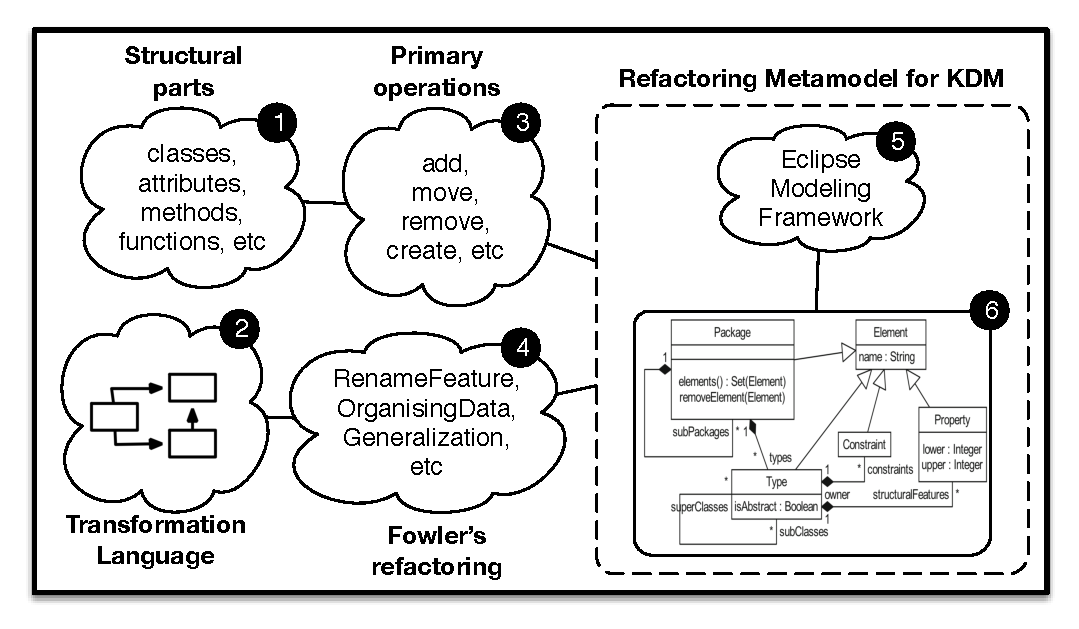
\includegraphics{figuras/ProcessoDOMetamodelo}}
\caption{Princípios e critérios utilizados para criar o metamodelo de refatoração para o KDM}
 \label{fig:processoDOMETAMODELO}
\end{figure}

\begin{figure}[h]
 \centering
 \scalebox{0.6}{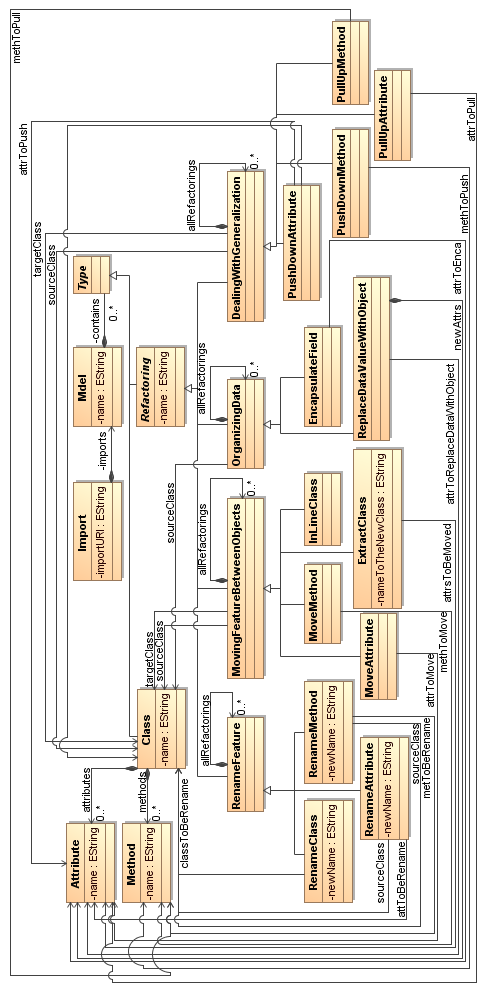
\includegraphics{figuras/metamodelo7}}
\caption{Metamodel de Refatoração para o KDM}
 \label{fig:METAMODELO}
\end{figure}

Para reutilizar a parte estrutural de uma refatoração, um modelo que represente essa estrutura é necessário. Para o exemplo \textit{RenameElement}, a estrutura basicamente consiste de uma \textit{metaclass} em um \textit{metamodel}. Outras refatorações, tais como \textit{ExtractClass} possuem restrições estruturais mais complexas, como a exigência de que a classe que será extraída esteja contida em um \textit{container object}. O metamodelo de refatorações para o KDM foi definido utilizado EMF (ver Figura~\ref{fig:processoDOMETAMODELO} \ding{186}). O metamodelo propriamente dito, Refac-KDM, pode ser visualizado na Figura~\ref{fig:METAMODELO}. As \textit{metaclasses} que compõem o metamodelo de refatoração, ou seja, Refac-KDM são definidas da seguinte forma:
 
\begin{itemize}

\item \textit{Refactoring} é o elemento raiz utilizado para armazenar todas as informações sobre as refatorações.

\item \textit{RenameFeature} corresponde às categorias de refatorações relacionadas a ação de renomear.\textit{RenameFeature} também armazena todas as refatorações relacionadas com a ação de renomear utilizando o \textit{metaattribute} \textit{allRefactorings}.

\item \textit{RenameClass} representa uma instância da refatoração \textit{rename Class}.  A semântica para a utilização da \textit{RenameClass} consiste em: (\textit{i}) especificar uma \textit{ClassUnit} (\textit{classToBeRenamed}), (\textit{ii}) bem como uma \textit{string} que representa o novo nome (\textit{newName}) da \textit{ClassUnit} após a aplicação da refatoração \textit{renameClassUnit}.

\item \textit{RenameAttribute} representa uma instância da refatoração \textit{rename Attribute}. A semântica para a utilização da \textit{metaclass} \textit{RenameAttribute} consiste em: (\textit{i}) especificar a \textit{ClassUnit} (\textit{sourceClass}) que armazena todos os atributos e todos os métodos, (\textit{ii}) o atributo que será renomeado (\textit{attToBeRename}) e (\textit{iii}) uma \textit{string} que representa o novo nome (\textit{newName}) do atributo após a aplicação da refatoração \textit{renameAttribute}.

\item \textit{RenameMethod} representa uma instância da refatoração \textit{rename Method}. A semântica para a utilização da \textit{metaclass} \textit{RenameMethod} consiste em: (\textit{i}) especificar a \textit{ClassUnit} (\textit{sourceClass}) que armazena todos os atributos e todos os métodos, (\textit{ii}) o método que será renomeado (\textit{methToBeRename}) e (\textit{iii}) uma \textit{string} que representa o novo nome (\textit{newName}) do método após a aplicação da refatoração \textit{renameMethod}.

\item \textit{MovingFeatureBetweenObjects} corresponde às categorias de refatorações relacionadas a ação de movimentar características entre objetos.

\item \textit{MoveAttribute} representa uma instância da refatoração \textit{move field}. A semântica para a utilização da \textit{metaclass} \textit{MoveAttribute} consiste em: (\textit{i}) especificar a \textit{ClassUnit} (\textit{sourceClass}) que armazena todos os atributos e todos os métodos, (\textit{ii}) a \textit{ClassUnit} (\textit{targetClass}) que irá receber o atributo a ser movido, (\textit{iii}) e o atributo que será movimentado (\textit{attrToMove}).  

\item \textit{MoveMethod} representa uma instância da refatoração \textit{move method}. A semântica para a utilização da \textit{metaclass} \textit{MoveMethod} consiste em: (\textit{i}) especificar a \textit{ClassUnit} (\textit{sourceClass}) que armazena todos os atributos e todos os métodos, (\textit{ii}) a \textit{ClassUnit} (\textit{targetClass}) que irá receber o método a ser movido, (\textit{iii}) e o método que será movimentado (\textit{methToMove}).

\item \textit{ExtractClass} representa uma instância da refatoração \textit{extract class}. A semântica para a utilização da \textit{metaclass} \textit{ExtractClass} consiste em especificar em: (\textit{i}) a \textit{ClassUnit} (\textit{sourceClass}) que armazena todos os atributos e todos os métodos, (\textit{ii}) uma lista de atributos (\textit{attrsToBeExtracted}) e uma lista de métodos (\textit{methsToBeExtracted}) para serem extraídos, (\textit{iii}) uma \textit{string} que representa o nome (\textit{newName}) da classe que foi extraída, (\textit{iv}) bem como um \textit{Package} (\textit{targetPackage}) que irá receber a classe criada após a execução da refatoração.

\item \textbf{TERMINAR AQUI TODAS AS METACLASSES}

\end{itemize} 

\subsubsection{Uma DSL para auxiliar a instânciação de refatorações com base no Refac-KDM}

A fim de utilizar plenamente as vantagens das refatorações, os desenvolvedores precisam ter um bom conhecimento de linguagem de programação avançada. Na verdade os desenvolvedores devem estar familiarizados como as semânticas das refatorações (por exemplo, qual(is) é (são) o(s) pré-requisito(s) para a execução de uma refatoração) e como/onde utilizar programar tais refatorações. A instanciação de uma refatoração utilizando o Refac-KDM é bastante verbosa, complexa e propensa a erros, uma vez que exige conhecimento avançadas de refatoração e habilidades avançadas de programação em relação a API Ecore. Com o objetivo de diminuir a quantidade de código-fonte, esforço e competência necessários para instanciar refatorações utilizando o Refac-KDM, foi desenvolvido uma linguagem especifica de domínio (do inglês, \textit{Domain-Specific Language} - DSL) que auxilia a instanciação de refatorações sistematicamente. 

A DSL para auxiliar a instanciação do Refac-KDM foi desenvolvida utilizando Xtext~\ref{sec:apoio_ferramental}\footnote{\texttt{https://www.eclipse.org/Xtext/}}. Xtext é um \textit{framework} do Eclipse\footnote{\texttt{https://www.eclipse.org}} que facilita a definição de gramática\footnote{Gramáticas representam a definição formal de um sintaxe textual concreta. Consistem em um conjunto de regras de produção para definir como o \textit{textual input} (, i.e., sentenças) são representadas. Basicamente, as regras de produção podem ser representadas utilizando \textit{Backus–Naur Form} (BNF), por exemplo, \textit{S ::= P1 ... Pn}, essa gramática define um símbolo \textit{S} por um conjunto de expressões \textit{P1 ... Pn}.} 
com o intuito de automatizar e agilizar o processo de desenvolvimento de DSLs.

 Em Xtext a gramática para especificar DSLs segue uma notação similar ao BNF chamada de \textit{parser rules}. Tais regras representam a sintaxe concreta da DSL. Note que para facilitar o entendimento da DSL, trechos da mesma são mostradas em listagens de códigos separados. Na listagem de código~\ref{lst:dsl_part_1} é ilustrado o primeiro trecho da gramática da DSL criada. 

\begin{lstlisting}[language=Xtext, frame=single, basicstyle={\scriptsize}, mathescape=true, label={lst:dsl_part_1}, caption={Gramática da DSL - parte 1}]
	
$\textrm{\ding{182}}$ grammar com.br.refactoring.xtext.Dsl with org.eclipse.xtext.common.Terminals 
$\textrm{\ding{183}}$ import ``platform:/resource/com.br.refactoring.dsl/model/kdm_refactoring.ecore'
$\textrm{\ding{184}}$ import ``http://www.eclipse.org/emf/2002/Ecore'' as ecore
Model: 
	$\textrm{\ding{185}}$ `model' name=ID
	$\textrm{\ding{186}}$ (imports+=Import)$^{*}$
	$\textrm{\ding{187}}$ (contains+=Type)$^{*}$
;
\end{lstlisting}

\begin{lstlisting}[language=Xtext, frame=single, basicstyle=\scriptsize, mathescape=true, label={lst:dsl_part_2}, caption={Gramática da DSL - parte 2}]
	$\textrm{\ding{182}}$ terminal ID: (`a'..`z' | `A'..`Z'|`_')(`a'..`z' | `A'..`Z'|`_'|`0'..`9')*;
\end{lstlisting}